\section{Constraints on lognormal bump}
In this last section we discuss the second type of constraints that we obtained. To begin with, we constrained the height of a lognormal bump placed at $k_\text{pk}=10$ Mpc$^{-1}$ using simulated data from the PIXIE experiment \cite{pixie}. We started producing a fiducial set of data from a power spectrum without the bump, then using \textbf{Montepython} we obtained 3 different types of constraints: the first one in which all the nuisance parameters presented in Table \ref{tab:nui_pixie}, a second one with a fixed foreground and a last one in which, by letting vary also $y_\text{reio}$, we marginalized over it.  In all the three cases we fixed the width of the bump at an intermediate value of $\sigma_\text{bump}=0.44$.\\
The analysis performed considering all the foreground nuisance parameters, shown in Figure \ref{fig:LN}, results in a constraint on the amplitude of the bump of $\mathcal{A}_\text{bump}<3.2\times10^{-2}$ at 95\% CL. This constraint becomes more stringent if we assume a perfect knowledge of the foreground parameters, as shown in Figure \ref{fig:LN_NN}, resulting in $\mathcal{A}_\text{bump}<7.7\times10^{-5}$. A milder constraint results instead if we marginalize only over $y_\text{reio}$, as shown in Figure \ref{fig:LN_NN_reio}, resulting in $\mathcal{A}_\text{bump}<4.0\times10^{-4}$.\\ 

\begin{figure}
    \centering
    \begin{subfigure}{0.49\textwidth}
        \centering
        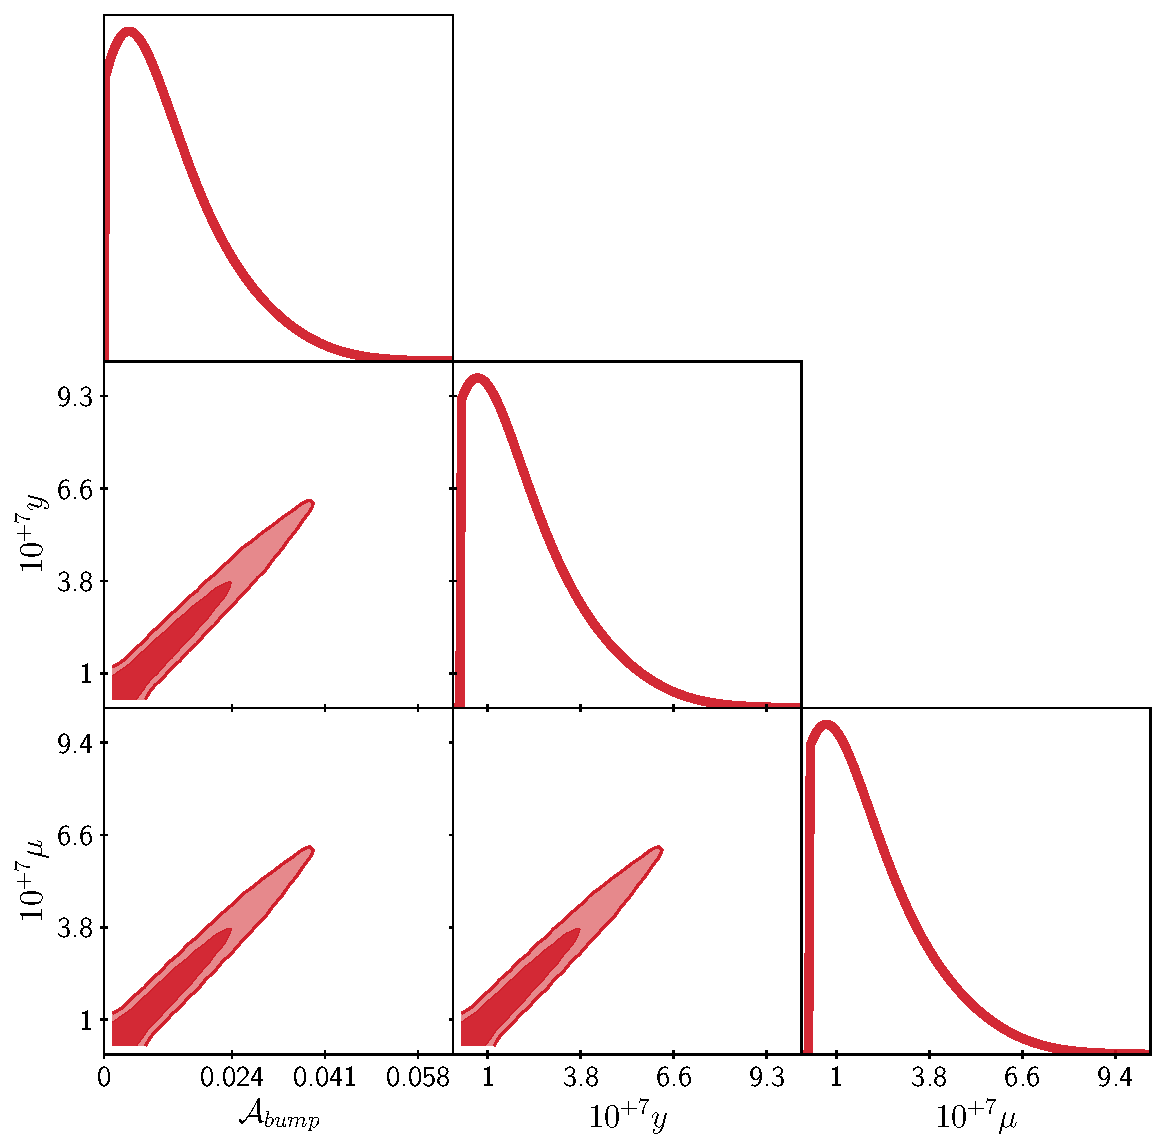
\includegraphics[width=0.7\textwidth]{Constraints/Lognormal.pdf}
        \caption{With nuisance}
        \label{fig:LN}        
    \end{subfigure}
    \hfill
    \begin{subfigure}{0.49\textwidth}
        \centering
        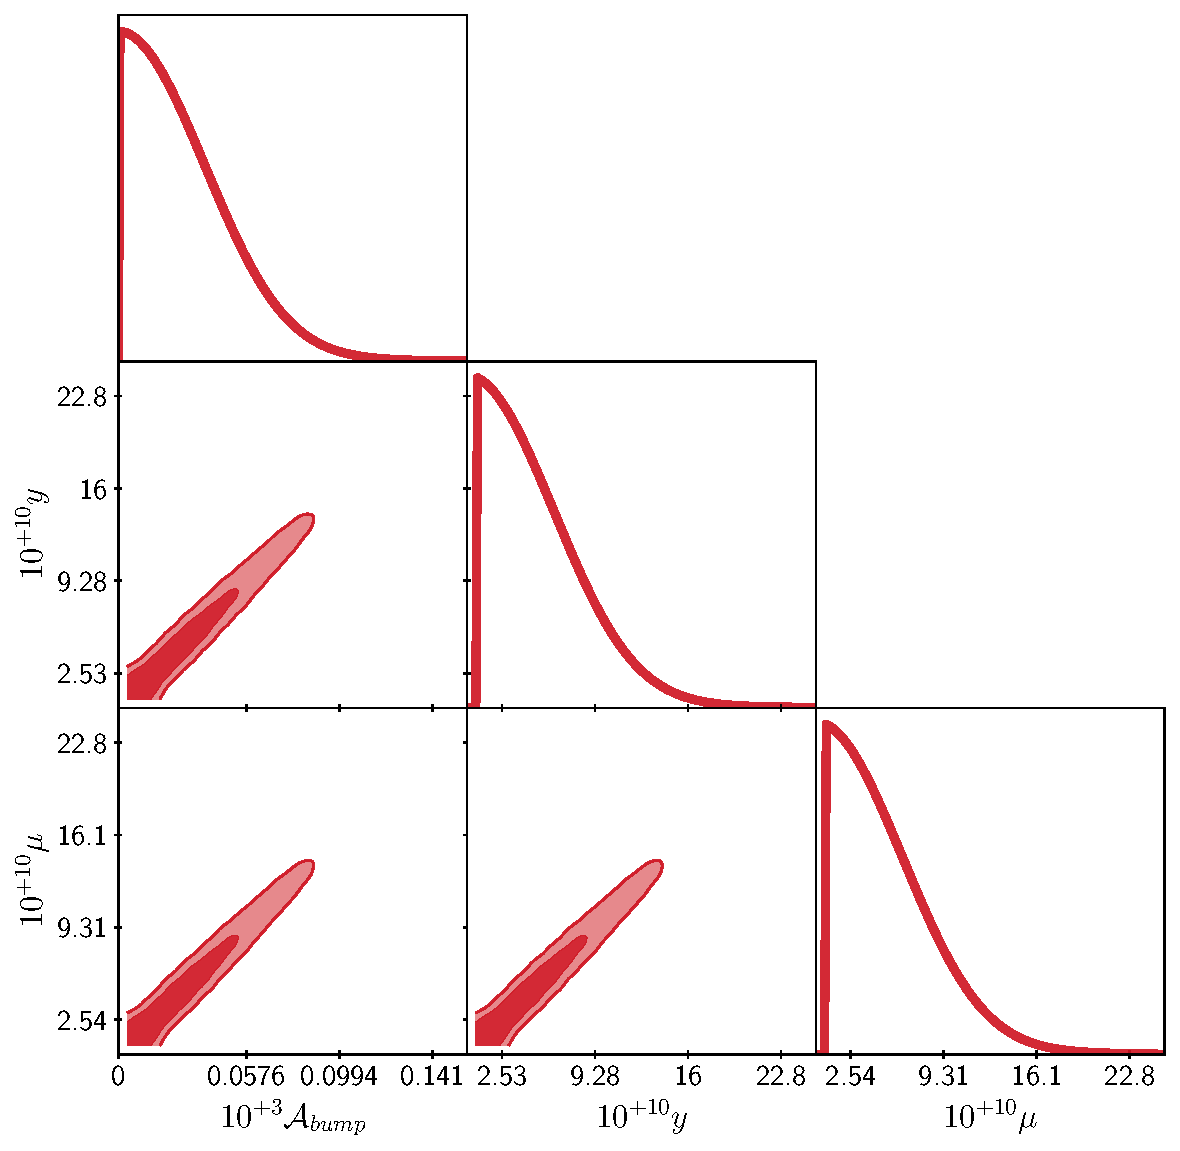
\includegraphics[width=0.7\textwidth]{Constraints/LN_NN.pdf}
        \caption{Without nuisance}
        \label{fig:LN_NN}        
    \end{subfigure}

    \vspace{1em}

    \begin{subfigure}{0.5\textwidth}
        \centering
        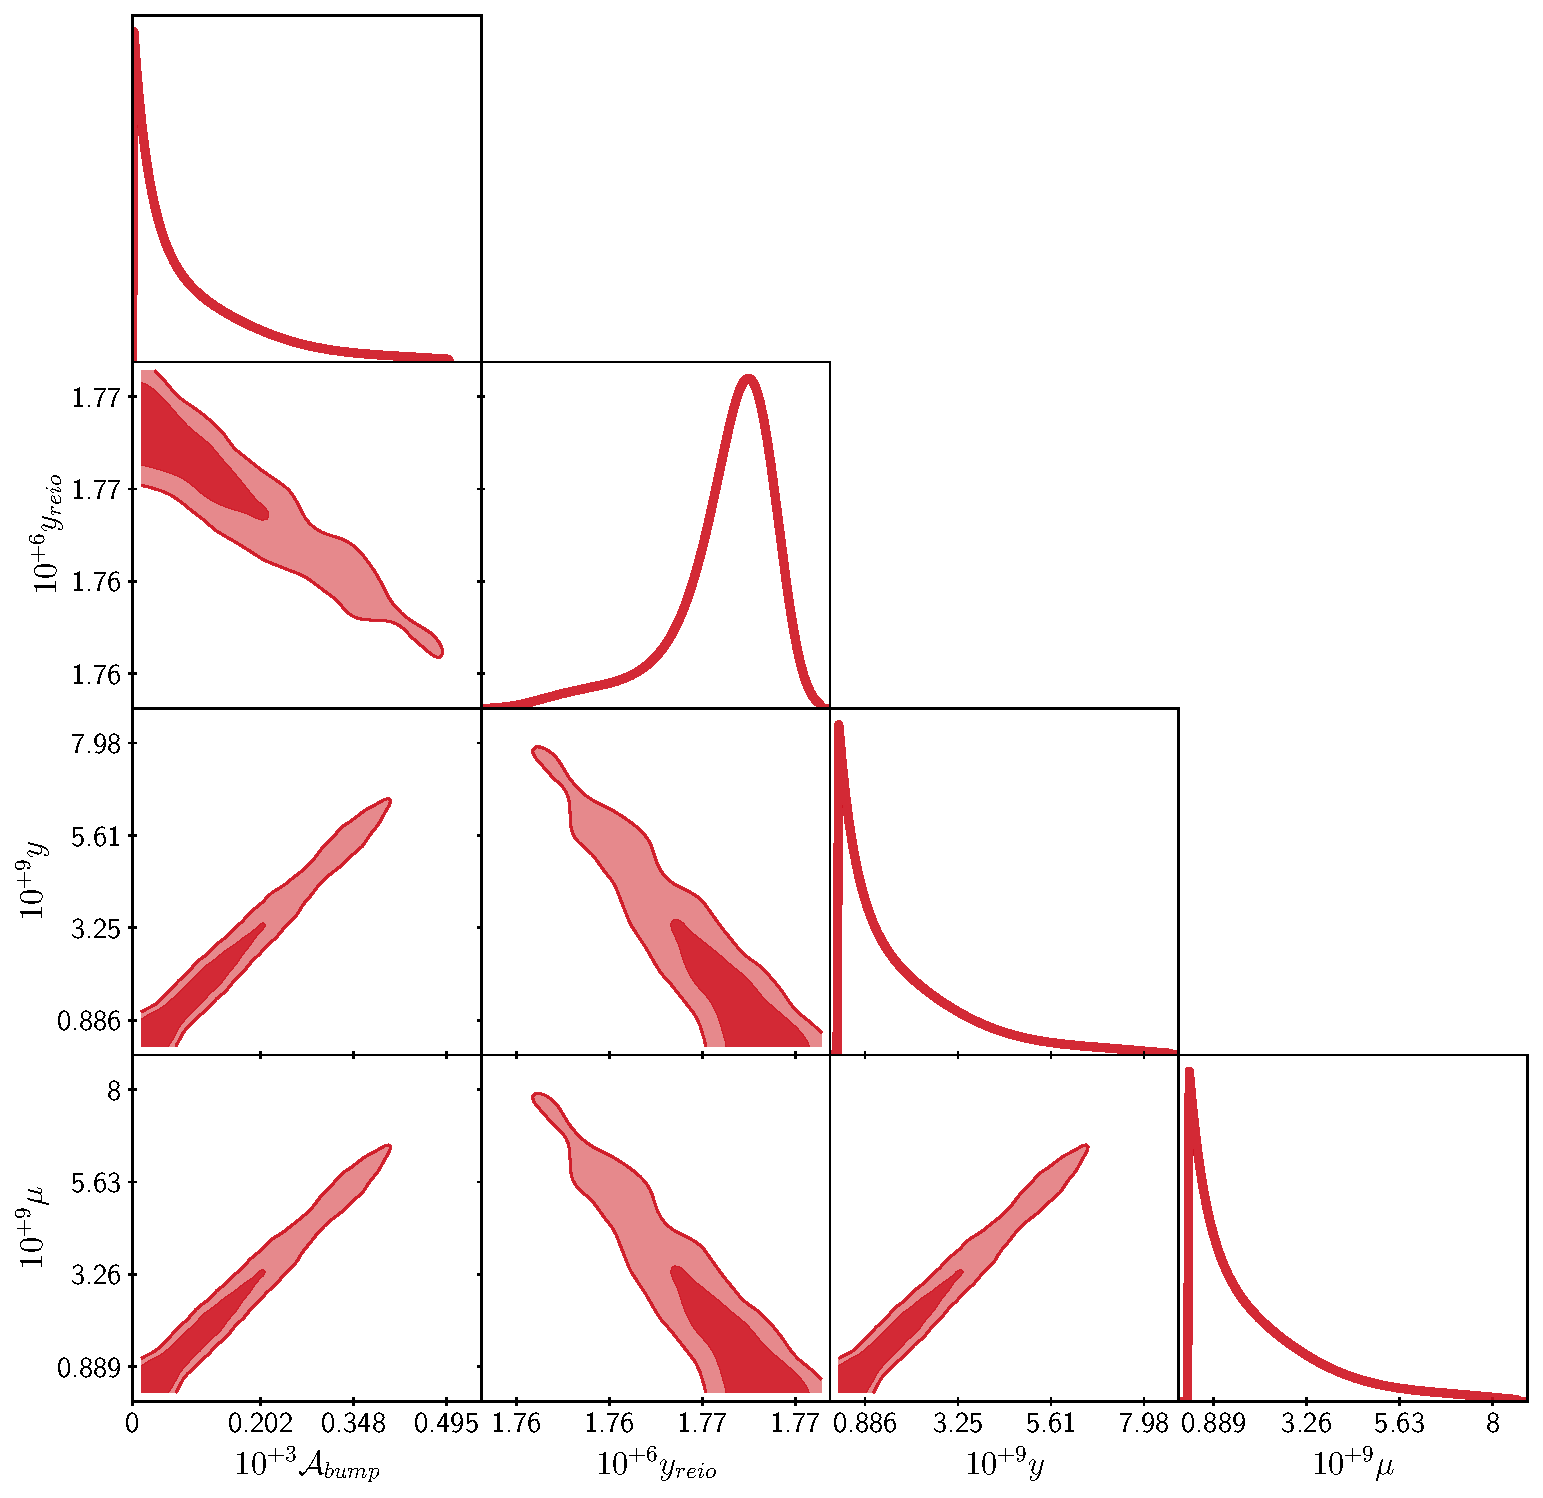
\includegraphics[width=0.7\textwidth]{Constraints/LN_NN_reio.pdf}
        \caption{Only $y_\text{reio}$ nuisance}
        \label{fig:LN_NN_reio}        
    \end{subfigure}
    \caption{Marginalized posterior distributions for the amplitude of a lognormal bump placed at $k_\text{pk}=10$ Mpc$^{-1}$ with width $\sigma_\text{bump}=0.44$. The three panels show the results obtained with different assumptions on the nuisance parameters.}
    \label{fig:LN_all}
\end{figure}


